\documentclass{beamer}

\usetheme{Madrid} % You can choose other themes like CambridgeUS, Madrid, etc.
\usepackage[utf8]{inputenc}
\usepackage[T1]{fontenc}
\usepackage{graphicx}
\usepackage{amsmath}
\usepackage{amssymb}
\usepackage{amsfonts}
\usepackage{booktabs} % For professional looking tables
\usepackage{subcaption} % Added based on the original document, though not directly used in the slides
\usepackage[autolanguage]{numprint}
\usepackage[style=ieee,backend=biber]{biblatex}
\addbibresource{../bibliography.bib} % your .bib file
\usepackage{float} % Added based on the original document, though not directly used in the slides
% \usepackage{booktabs} % This was a duplicate, removed.

% Load hyperref ONCE with all options
% \usepackage[colorlinks=true,        % Enables colored links
%             linkcolor=blue,         % Color for internal links (e.g., table of contents)
%             citecolor=blue,         % Color for citation links
%             urlcolor=blue,          % Color for URLs
%             breaklinks=true,        % Allows links to break over lines
%             bookmarks=true,
%             bookmarksdepth=3]{hyperref}

\usepackage{ragged2e} % For \justifying
\usepackage{fontawesome5}
% Acronyms (re-define for presentation context if needed, or just use full names)
\usepackage[nolist]{acronym}
\begin{acronym}
  \acro{EQA}[EQA]{Extractive Question Answering}
  \acro{NLP}[NLP]{Natural Language Processing}
  \acro{GAI}[GAI]{Generative Artificial Intelligence}
  \acro{QA}[QA]{Question Answering}
  \acro{AI}[AI]{Artificial Intelligence}
  \acro{LLMs}[LLMs]{Large Language Models}
  \acro{DL}[DL]{Deep Learning}
  \acro{LNLP}[LNLP]{Legal NLP}
  \acro{LQA}[LQA]{Legal Question Answering}
  \acro{RNNs}[RNNs]{Recurrent Neural Networks}
  \acro{LSTM}[LSTM]{Long Short-Term Memory}
  \acro{CNN}[CNN]{Convolutional Neural Networks}
  \acro{TF-IDF}[TF-IDF]{Term Frequency-Inverse Document Frequency}
  \acro{SQuAD}[SQuAD]{Stanford Question Answering Dataset}
  \acro{NER}[NER]{Named Entity Recognition}
  \acro{LDS}[LDS]{Legal Document Summarization}
  \acro{SVM}[SVM]{Support Vector Machine}
  \acro{GQA}[GQA]{Generative Question Answering}
\end{acronym}

% Show section title at the beginning of each section
\AtBeginSection[]{
  \begin{frame}
    \centering
    \vfill
    \begin{beamercolorbox}[sep=12pt,center,shadow=true,rounded=true]{title}
      \usebeamerfont{title}\insertsectionhead
    \end{beamercolorbox}
    \vfill
  \end{frame}
}

\title[Transformer Models for EQA]{Leveraging Transformer Models for Extractive Question Answering in Criminal Report Analysis}
\author[Falconi et al.]{Lenin G. Falconi \and Lorena Isabel Barona-López \and \\Myriam Hernandez-Alvarez}
\institute[DICC, EPN]{Departamento de Informática y Ciencias de la Computación (DICC), \\Escuela Politécnica Nacional, Ecuador}
\date{July 21, 2025}

\begin{document}

\justifying % Justify text for better readability

% {
% \setbeamertemplate{footline}{} % No footline on title page
% \begin{frame}
%     \titlepage
% \end{frame}
% }

% Title Slide
\titlegraphic{
  \includegraphics[width=1.5cm]{./figures/logoEPN.jpg}
}
\begin{frame}
    \titlepage
\end{frame}

% Table of Contents
\begin{frame}
    \frametitle{Overview}
    \tableofcontents
  \end{frame}
  
\section{Introduction}
\label{sec:introduction}

\begin{frame}
    \frametitle{Introduction: The Problem}

    \begin{columns}
      \begin{column}{.4\textwidth}

          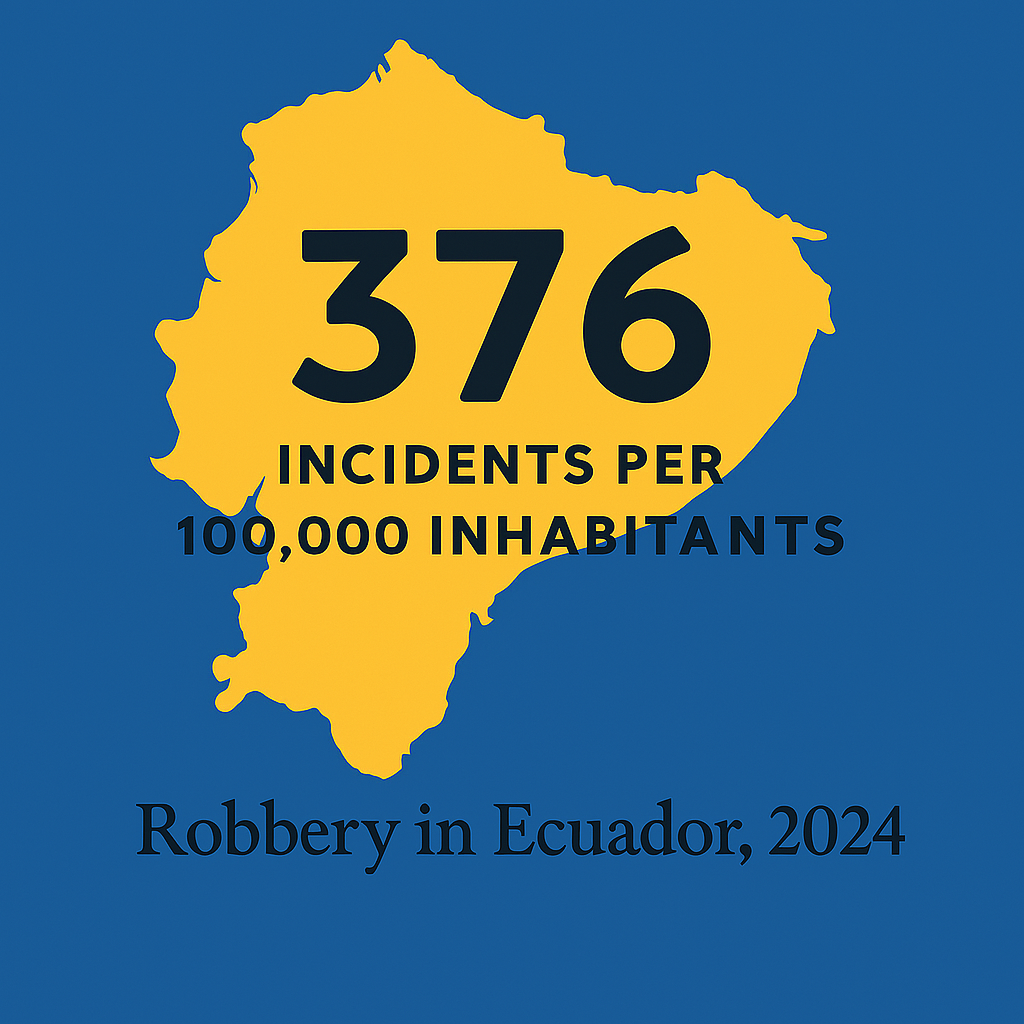
\includegraphics[width=\textwidth]{./figures/robbery-rate2.png}

        \end{column}
        \begin{column}{.6\textwidth}

              \begin{itemize}
              \item \textbf{Context:} Ecuadorian Prosecutor's Office
                handled $\numprint{67705}$ robbery incidents in 2024.
              
              \item \textbf{Need:} Efficient extraction of information
                from criminal reports for:
                \begin{itemize}
                \item More effective investigations.
                \item Supporting victims' insurance claims.
                \item Providing data for public safety planning.
                \end{itemize}
              \item \textbf{Goal:} Adapt Transformer-based
                models for \ac{EQA} in Ecuadorian legal documents
                about robbery.
    \end{itemize}

     \end{column}

\end{columns}

\end{frame}

\begin{frame}
    \frametitle{Our Contribution}
    \begin{itemize}
    \item \faLaptopCode\ \textbf{Domain-Adapted BERT model:} First
      application of transformer-based models for \ac{EQA} on
      Spanish-language robbery case reports from Ecuador.
    \item \faDatabase\ \textbf{Novel Dataset:} using \ac{GAI} to
      curate a Spanish-language \ac{SQuAD} dataset derived from
      Ecuadorian legal documents.
    \item \faServer\ \textbf{Potential Impact:} Enhance information
      retrieval within judicial systems and optimize workloads,
      improving service delivery to communities.
    \end{itemize}
\end{frame}

\section{Related Works}
\label{sec:related-works}

% \begin{frame}
%     \frametitle{Introduction: Purpose of Literature Review}
%     \begin{itemize}
%         \item Explores the landscape of \ac{AI} applications in \ac{NLP}, with a specific focus on legal domains.
%         \item Identifies the current state-of-the-art in Question Answering (\ac{QA}) using Transformer models.
%         \item Highlights the gap in research concerning domain-adapted Transformer models for Spanish legal texts.
%     \end{itemize}
% \end{frame}

\begin{frame}
    \frametitle{Large Language Models (\ac{LLMs}) \& Generative AI (\ac{GAI})}
    \framesubtitle{Foundational Concepts}
    \begin{itemize}
        \item \textbf{\ac{LLMs}:} A subset of Foundational \ac{AI} and \ac{GAI} models, primarily text-based.
        \begin{itemize}
            \item Leverage transformer architectures \cite{Minaee2025,Grattafiori2024}.
            \item Undergo extensive pre-training on textual corpora.
            \item Exhibit strong natural language understanding and problem-solving capabilities.
        \end{itemize}
      \item \textbf{\ac{GAI}:} aims to learn a model distribution
        $p_{model}(\mathbf{x})$ that approximates the true data
        distribution $p_{data}(\mathbf{x})$, where $\mathbf{x}$
        represents observations from the data domain \cite{Grattafiori2024}. 

\begin{equation}
  \label{eq:gai-def}
  p_{model}(\mathbf{x}) \approx p_{data}(\mathbf{x})
\end{equation}
    \end{itemize}
\end{frame}

\begin{frame}
    \frametitle{Question Answering (\ac{QA}) in Legal Contexts}
    \framesubtitle{Complexity and Approaches}
    \begin{itemize}
        \item \textbf{\ac{LQA}:} Complex task requiring analysis and nuanced interpretation of extensive legal corpora \cite{Ariai2024}.
        \item \textbf{Traditional \ac{QA} Methods:}
        \begin{itemize}
            \item \ac{RNNs}, \ac{LSTM}, \ac{CNN}.
            \item Information retrieval approaches like \ac{TF-IDF}.
        \end{itemize}
        \item \textbf{Modern \ac{QA} Paradigms:}
            \begin{itemize}
                \item \textbf{\ac{EQA}:} Identifies and retrieves a direct text span from context.
                \item \textbf{\ac{GQA}:} Synthesizes responses using encoder-decoder architectures.
            \end{itemize}
    \end{itemize}
\end{frame}

\begin{frame}
    \frametitle{EQA vs. GQA: Key Distinctions}
    \begin{table}[h]
        \centering
        \small
        \caption{Comparison of EQA and GQA Approaches}
        \label{tab:eqa-gqa-comparison}
        \begin{tabular}{p{0.2\textwidth}p{0.35\textwidth}p{0.35\textwidth}}
            \toprule
            \textbf{Feature} & \textbf{\ac{EQA} (Extractive)} & \textbf{\ac{GQA} (Generative)} \\
            \midrule
            \textbf{Output} & Direct text span from context & Synthesized, novel response \\
            \textbf{Architecture} & Predicts start/end positions & Encoder-decoder \\
            \textbf{Context Length} & More effective with limited context & Generally outperforms with longer contexts \\
            \textbf{Fluency} & Less fluent (direct extraction) & More fluent and comprehensive \\
            \textbf{Generalization} & Better out-of-domain generalization & Can be limited by training data \\
            \bottomrule
        \end{tabular}
        \vspace{0.2cm}
        \justifying \footnotesize \textit{Source: Adapted from Luo et al. \cite{Luo2022NLP}}
    \end{table}
\end{frame}

\begin{frame}
    \frametitle{Related Works: AI in Legal Domains}
    \framesubtitle{State-of-the-Art Applications}
    \begin{itemize}
        \item Significant interest in applying \ac{AI} to legal fields, with transformers leading in \ac{NLP} tasks.
        \item \textbf{RoBERTa for Legal \ac{QA}:} \cite{Vold_Conrad_2021} showed RoBERTa outperforming \ac{SVM} for legal questions (31\% F1-score improvement).
        \item \textbf{Transformer-based Answer Selection:} \cite{Shao_Guo_Chen_Zepeng_2019} demonstrated effectiveness in general \ac{QA} by extracting global information.
        \item \textbf{Legal Information Retrieval:} \cite{Kim_Rabelo_Babiker_Rahman_Goebel_2024} utilized sentence-transformers for case law retrieval and fine-tuned DeBERTa for legal entailment.
    \end{itemize}
\end{frame}

\begin{frame}
    \frametitle{Related Works: AI in Legal Domains (Cont.)}
    \framesubtitle{Predicting Judgments \& Text Generation}
    \begin{itemize}
        \item \textbf{Predicting Legal Judgments:} \cite{Ghosh_Kumar_2024} evaluated six transformer models (BERT, XLNet, RoBERTa, DeBERTa, ELECTRA, BigBird) for legal judgment prediction, achieving up to 80\% accuracy.
        \item \textbf{Generating Legal Text:} \cite{Peric_Mijic_Stammbach_Ash_2020} explored transformers for generating judicial opinions and distinguishing human vs. machine-generated legal texts, beneficial for drafting.
    \end{itemize}
\end{frame}

\begin{frame}
    \frametitle{Novelty of the Current Study}
    \begin{itemize}
        \item The literature review identifies a critical research gap.
        \item Our study introduces a novel application of transformer-based models that:
        \begin{itemize}
            \item Simultaneously addresses \textbf{Spanish language} texts.
            \item Focuses specifically on \textbf{legal documents} (criminal reports).
        \end{itemize}
        \item This combination fills a unique niche, contributing new insights to \ac{LNLP}.
    \end{itemize}
\end{frame}

\begin{frame}
    \frametitle{Key Literature Insights}
    \begin{itemize}
        \item \ac{LLMs} and \ac{GAI} are foundational for advanced \ac{NLP}, including legal applications.
        \item Both \ac{EQA} and \ac{GQA} have distinct strengths, with \ac{EQA} being suitable for precise information extraction from defined contexts.
        \item Transformer models have shown superior performance across various legal \ac{NLP} tasks, from \ac{QA} to judgment prediction and text generation.
        \item Our research uniquely combines Spanish language processing with legal domain adaptation using transformers, addressing a previously unexplored area.
    \end{itemize}
  \end{frame}

\section{Methodology}
\label{sec:methodology}

\begin{frame}
  \frametitle{Methodology Overview}
  \centering
  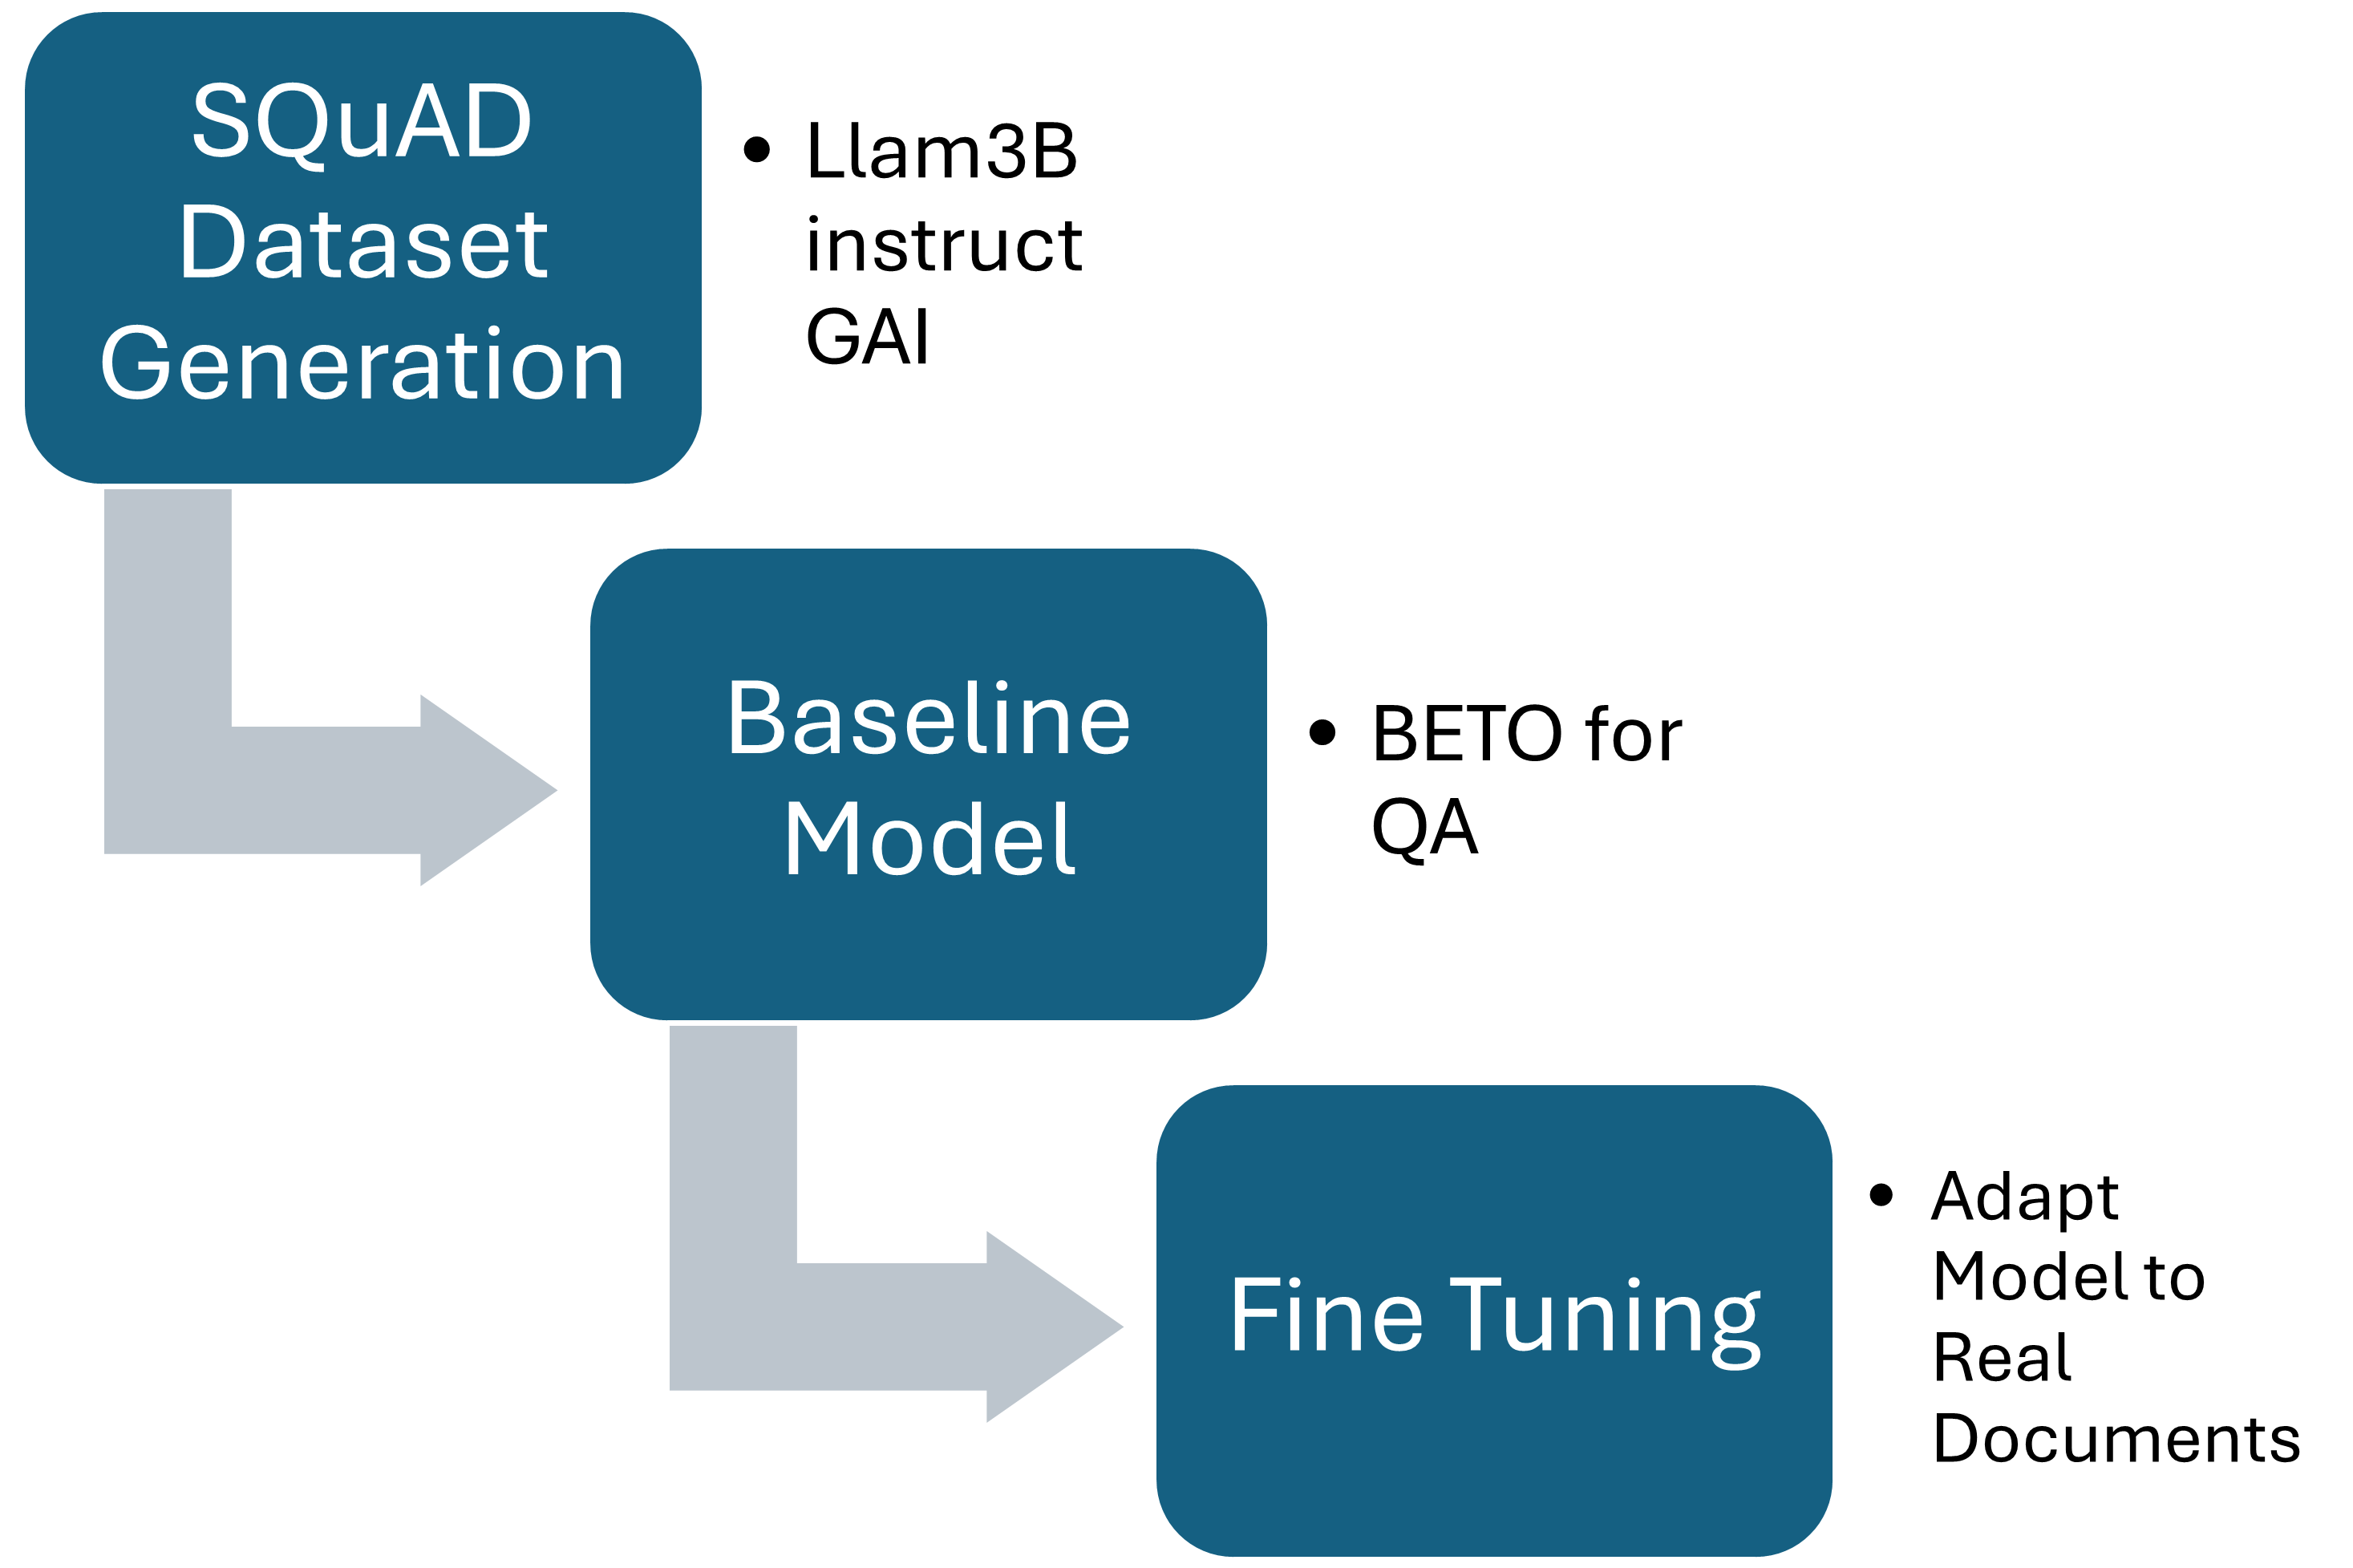
\includegraphics[width=0.8\textwidth]{./figures/methodology.png}


\end{frame}

\begin{frame}
    \frametitle{Methodology Overview}
    Our methodology consists of three phases:
    \begin{enumerate}
        \item \textbf{Dataset Generation:} Creation of a domain-specific \ac{SQuAD}-format dataset using \ac{GAI}.
        \item \textbf{Baseline Model Performance:} Evaluation of a pre-trained BERT model on this dataset.
        \item \textbf{Model Fine-Tuning:} Adaptation of the BERT model to robbery reports.
    \end{enumerate}
\end{frame}

\begin{frame}
  \frametitle{Phase 1: Robbery Crime \ac{QA} Dataset Generation}
  \centering
  
\includegraphics[width=.9\textwidth]{./figures/methodology2.png}
\end{frame}
\begin{frame}[allowframebreaks]
    \frametitle{Phase 1: Robbery Crime \ac{QA} Dataset Generation}
    \framesubtitle{Data Collection and Preprocessing}
    \begin{itemize}
        \item Constructed dataset from unlabeled Spanish robbery crime reports.
        \item Preprocessing: Removed non-alphanumeric characters, converted to lowercase.
        \item Filtered reports $x_i$ with word counts $82 \leq \Gamma(x_i) \leq 150$ to remove outliers.
        \item Transformed into \ac{SQuAD}-compatible format using \ac{GAI}.
    \end{itemize}
    % Figures from the paper (placeholder, as actual image files are not provided)
    \begin{figure}
        \centering
        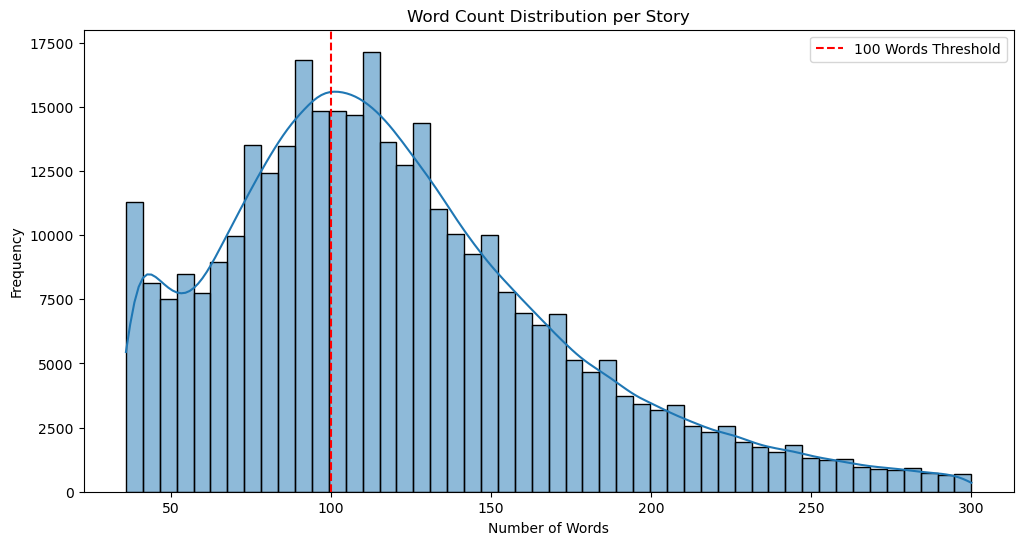
\includegraphics[width=0.7\textwidth]{../images/histogramOriginalDataset.png}
        \caption*{Distribution of word counts (Histogram)}
    \end{figure}
\end{frame}

\begin{frame}
    \frametitle{Phase 1: Robbery Crime \ac{QA} Dataset Generation}
    \framesubtitle{Generative \ac{AI} Prompt Engineering}
    \begin{itemize}
        \item Used \textbf{Meta-Llama-3-8B-Instruct} for dataset creation.
        \item \ac{LLMs} acted as an expert data science assistant to construct a Spanish \ac{SQuAD} dataset.
        \item Prompt received \texttt{context} (crime report) and \texttt{question} (from predefined list).
        \item Output in \texttt{json} format: \texttt{context}, \texttt{question}, \texttt{answer\_text}, \texttt{answer\_start}, \texttt{answer\_end}, \texttt{impossible\_find\_answer}.
    \end{itemize}
\end{frame}

\begin{frame}
    \frametitle{Phase 1: Robbery Crime \ac{QA} Dataset Generation}
    \framesubtitle{Proposed Questions for the Dataset}
    \begin{table}[h]
      \centering
      \small
    \caption{Proposed Questions for the Dataset}
    \label{tab:commonquestions-slide}
    \begin{tabular}{|p{0.9\textwidth}|}
    \hline
    \textbf{Question} \\
    \hline
    What objects were stolen? \\
    On what date did the incident occur? \\
    At what time did the robbery happen? \\
    At what address or between which streets did the robbery/incident occur? \\
    What was the dollar value of the stolen or taken objects? \\
    \hline
    \end{tabular}
    \end{table}
    \begin{itemize}
        \item Initial $\numprint{1544}$ samples generated $\numprint{7705}$ question-answer pairs.
        \item Identified $\approx \numprint{3000}$ invalid cases using \texttt{impossible\_find\_answer} flag.
        \item Final curated dataset: $\numprint{4572}$ samples (answer length $\leq 17$ words).
    \end{itemize}
\end{frame}

\begin{frame}
    \frametitle{Phase 1: Robbery Crime \ac{QA} Dataset Generation}
    \framesubtitle{Dataset Train and Test Split}
    \begin{itemize}
        \item Random split: 80\% for training, 20\% for testing.
        \item Ensures evaluation of model's generalization capability.
    \end{itemize}
    \begin{table}[htbp]
    \caption{Dataset Train and Test Split}
    \centering
    \small
    \begin{tabular}{lr}
      \toprule
    Partition & \# Samples\\
    \midrule
    Train & $\numprint{3657}$\\
      Test & $\numprint{915}$\\
      \midrule
      Total & $\numprint{4572}$\\
      \bottomrule
    \end{tabular}
    \end{table}
\end{frame}

\begin{frame}
    \frametitle{Phase 2: Baseline Model Architecture and Performance}
    \begin{itemize}
        \item \textbf{Model Selected:} \texttt{mrm8488/bert-base-spanish-wwm-cased-finetuned-spa-squad2-es}
        \item Distilled version of BETO (Spanish BERT), fine-tuned on SQuAD-es-v2.0.
        \item \textbf{Architecture (BERT-base configuration):}
        \begin{itemize}
            \item 12 Transformer blocks
            \item 768-dimensional hidden states
            \item 12 self-attention heads
            \item 384 tokens of sequence length
        \end{itemize}
        \item \textbf{Baseline Performance (without additional fine-tuning):} F1-score of 81.70.
    \end{itemize}
\end{frame}

\begin{frame}
    \frametitle{Phase 3: Model Fine-Tuning}
    \begin{itemize}
        \item All layers are trained.
        \item Recalculation of start/end indices.
        \item Truncation applied to context (128-token window) for long texts.
        \item Small learning rate recommended for fine-tuning to adapt pre-trained knowledge.
    \end{itemize}
    \begin{table}[htbp]
    \caption{Training Parameters}
    \centering
    \small
    \begin{tabular}{ll}
      \toprule
    Parameter & Value\\
    \midrule
    Strategy & epoch\\
    Learning rate & $2 \times 10^{-5}$\\
    Batch Size & 64\\
    Epochs & 10\\
    Weight Decay & 0.01\\
    FP16 & True\\
      Metric for best model & F1 (eval)\\
      \bottomrule
    \end{tabular}
    \end{table}
\end{frame}

\section{Experimental Results}
\label{sec:experimental-results}


\begin{frame}
    \frametitle{Results: Model Performance}
    \framesubtitle{Pre-trained Model Performance (Baseline)}
    \begin{table}[h]
      \centering
      \small
      \caption{Pre-trained Model Performance}
      \label{tab:before-performance-slide}
      \begin{tabular}{lr}
    \toprule
    Metric & Value \\
    \midrule
    eval\_loss & 0.9102 \\
    eval\_exact & 53.5519 \\
    eval\_f1 & 81.7041 \\
    eval\_total & 915.0000 \\
    eval\_HasAns\_exact & 53.5519 \\
    eval\_HasAns\_f1 & 81.7041 \\
    eval\_HasAns\_total & 915.0000 \\
    \bottomrule
    \end{tabular}
    \end{table}
\end{frame}

\begin{frame}
    \frametitle{Results: Model Performance}
    \framesubtitle{Fine-Tuned Model Performance}
    \begin{table}[h]
      \centering
      \small
      \caption{Fine-Tuned Model Performance}
      \label{tab:finetunedModel-slide}
      \begin{tabular}{lr}
    \toprule
    Metric & Value \\
    \midrule
    eval\_loss & 1.0088 \\
    eval\_exact & 55.7377 \\
    eval\_f1 & \textbf{82.8805} \\
    eval\_total & 915.0000 \\
    eval\_HasAns\_exact & 55.7377 \\
    eval\_HasAns\_f1 & \textbf{82.8805} \\
    eval\_HasAns\_total & 915.0000 \\
    epoch & 10.0000 \\
    \bottomrule
    \end{tabular}
    \end{table}
    \begin{itemize}
        \item \textbf{Improvement:} Fine-tuned model achieved an F1 score of \textbf{82.88}, outperforming the pre-trained baseline of 81.70.
        \item Demonstrates effectiveness of domain-specific fine-tuning.
    \end{itemize}
\end{frame}

\section{Conclusions and Future Work}
\label{sec:conclusions}


\begin{frame}
    \frametitle{Conclusions}
    \begin{itemize}
    \item Demonstrated the effectiveness of transformer-based models
      for \ac{EQA} in criminal report analysis.
    \item Fine-tuned model showed notable improvement (F1 score of
      82.88) over the pre-trained model (81.70).
    \item Model can facilitate extraction of crucial information,
      supporting legal practitioners.
    \item Proposed Methodology can be used to fine tune models for
      \ac{LQA} in other languages.
    \end{itemize}
\end{frame}

\begin{frame}
    \frametitle{Limitations and Future Work}
    \begin{itemize}
        \item \textbf{Limitations:} Occasional inability to retrieve accurate answers, need for manual verification of results.
        \item \textbf{Future Work:}
        \begin{itemize}
            \item Explore additional advanced techniques.
            \item Incorporate manual labeling by expert peers to improve dataset quality.
            \item Utilize additional computational resources for larger datasets.
            \item Investigate other \ac{NLP} techniques in Ecuadorian
              legal context (e.g., Legal \ac{NER}, Legal Document
              Summarization).
            \item  Study the proposed methodology in other languages.
        \end{itemize}
        \item \textbf{Overall Goal:} Harness the full potential of \ac{AI} in supporting the justice system for more efficient case management and resource allocation.
    \end{itemize}
\end{frame}

\begin{frame}
    \frametitle{Acknowledgements}
    \begin{itemize}
        \item Faculty of Systems Engineering at Escuela Politécnica Nacional, Quito, Ecuador (academic guidance and financial support).
        \item Fiscalía General del Estado (cooperation in research development).
    \end{itemize}
    \textbf{Declaration of Competing Interests:} The authors have no competing interests to declare.
\end{frame}

\begin{frame}
  \frametitle{Thanks}
  
\includegraphics[width=\textwidth]{./figures/thanks.jpg}
\end{frame}
% Bibliography
\begin{frame}[allowframebreaks]
    \frametitle{References}
    % \nocite{*} % This command will include all entries from your .bib file
    \printbibliography
\end{frame}
\end{document}
%%% Local Variables:
%%% mode: LaTeX
%%% TeX-master: t
%%% End:
